\chapter{基于跳数的启发式距离向量算法}
\label{chap:基于跳数的启发式距离向量算法}

本章提出一种用于机会网络的基于跳数的启发式距离向量算法HCH,主要贡献如下:

\begin{enumerate}
\item 设计了启发函数用以预测消息投递所需跳数。启发策略所需的信息由节点间传递的消息数据包携带。
\item 形式化定义了矩阵运算,从而将跳数预测计算转化为矩阵运算。
\item 利用ONE模拟器对HCH算法进行了仿真,结果表明HCH具有较高的投递率以及较低的投递时延,且网络开销保持在可接受水平。
\end{enumerate}

本章组织如下:\ref{chap5:系统模型}节中介绍了系统模型及路由模型;\ref{chap5:消息投递跳数预测}节中提出了跳数预测算法;\ref{chap5:路由协议}节中提出了基于跳数的启发式距离向量路由算法;\ref{chap5:仿真实验}节为仿真实验;\ref{chap5:本章小结}节概括了本章内容。


\section{系统模型}
\label{chap5:系统模型}

在该模型中,网络包含一组移动节点,节点之间对等通信。基本假设如下:
\begin{itemize}
\item 所有节点以对等方式通信,即网络中不存在任何辅助消息进行传递的基础设备。换言之,不存在路由器类似的设备用于转发消息,所有的节点合作以多跳的方式进行消息投递,节点自身将做出对消息的转发决策。
\item 节点的移动方式多变难以预测,即难以对某个节点预测其下一时间或下一时间段的路径及地点。
\end{itemize}

数学符号如\tablename~\ref{tab:chap5_math_table}所示。节点集合以$V=\{v|1\leq v\leq n\}$表示。为便于分析,描述路由的过程只针对某一条消息而言,并以$s$代表其源节点,$d$代表其目的节点,该消息用符号$M_k(s,d)$表示,其索引号为$k$。符号$hop(k)$为一个整数,表述消息$M_k$所经过的跳数值。符号$\overline{hop}(i,j)$表示消息从节点$i$到达节点$j$之间的平均跳数。

在此模型下,本章解决如下问题:
\begin{itemize}
\item 如何设计效用指标衡量网络当前状态
\item 如何从网络中收集信息,从而动态计算效用指标
\item 如何根据效用值选择节点的转发策略
\end{itemize}



\begin{table}[tbp]
  \caption{数学符号定义}
  \label{tab:chap5_math_table}
\centering
  \begin{tabular}{p{0.15\linewidth}<{\centering}p{0.73\linewidth}<{\centering}}
  \hline
   \textbf{notation} & \textbf{meaning}  \\
    \hline
    $n$ & 节点总数\\ 
    $V$ & 节点集合(|V|=n)\\ 
    $M_k(s,d)$ & 索引号为 $k$的消息,其中源节点为$s$,目的节点为$d$\\   
    $\overline{hop}(i,j)$ & 节点 $i$ 和节点$j$之间的平均跳数 \\ 
    $hop(k)$ & 消息 $M_k$ 当前经过的跳数\\
    $h(i,j)$ & 节点 $i$ 和 $j$之间的估计跳数 \\
    \hline
  \end{tabular}
\end{table}


\section{消息投递跳数预测}
\label{chap5:消息投递跳数预测}

在本节中,定义了用于路由决策的效用函数,即投递消息所需跳数的预测值。首先讨论如何从网络中收集所需信息。然后基于收集到的信息提出启发函数。路由协议的转发决策将由该函数决定。

\subsection{消息收集}
\label{chap5:消息收集}

在提出的算法中,利用了消息跳数指标来做出路由决策。跳数信息有很多方式获取,本章中的方法,即是令网络中的消息数据包头部携带有该消息所进过的节点的记录。当某消息数据包到达一个节点时,该节点将获得该消息所经过的节点到该节点所经过的条数值。例如,若消息$M_k$产生于节点$s$,并沿路径$s\rightarrow p\rightarrow q\rightarrow r$转发,则从该消息的头部,节点$r$可以获知:节点$s$与节点$r$之间为3跳,$p$与$r$之间为2跳,$q$与$r$之间为1跳。这些记录是针对消息$M_k$而言的,若对节点$r$所收到的所有消息的对应记录求平均值,则得到这些节点到$r$的平均跳数;在本章中,利用滑动窗口方法实现该目的。每个节点维护一个矩阵,记为$\bm{A}$,用于记录其它所有节点到该节点的跳数值。每个矩阵元素将对应一个滑动窗口。

\figurename~\ref{fig:chap5_matrix}为矩阵$\bm{A}$及其每个元素所对应的滑动窗口工作方式。对于矩阵$\bm{A}$中的每个元素,都有一个对应的滑动窗口记录了之前收到的消息对应的跳数信息。滑动窗口越长,则对网络状态的变化越不敏感,反之则越敏感。通过对滑动窗口中记录的跳数值,即从$t-r+1$到$t$位置取平均,则得到该矩阵元素对应节点到当前节点的平均跳数。由此得到跳数预测值,记为$a(t+1)$。

\begin{figure}[bt]
  \centering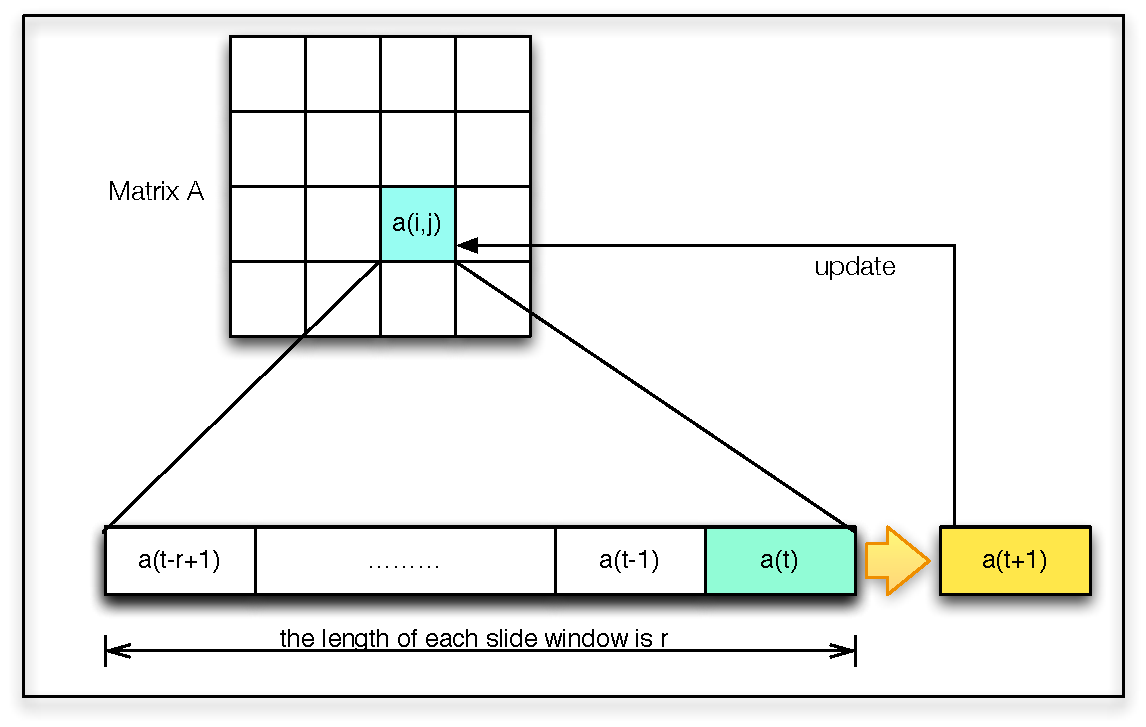
\includegraphics[width=0.7\textwidth]{paper-HCH/matrix}
  \caption{矩阵$\bm{A}$及其对应的滑动窗口}
  \label{fig:chap5_matrix}
\end{figure}

\begin{algorithm}[tbp] %算法的开始
\caption{Maintaining the matrix $\boldmath{A}$ and its slide-windows} %算法的标题
\label{alg:chap5_matrix} %给算法一个标签,这样方便在文中对算法的引用
\begin{algorithmic}[1] %这个1 表示每一行都显示数字
\REQUIRE  %算法的输入参数:Input
packet $M_k$, current time $t+1$
\ENSURE  %算法的输出:Output
matrix $\boldmath{A}$, slide-window $win$ \\
When packet $M_k$ comes\\
\textbf{local variables:} $i,j,c$
\STATE $i\leftarrow M_k.getSourceNodeID()$
\STATE $Sequence\leftarrow M_k.getPassedNodes()$
\STATE $c\leftarrow 1$
\FOR{$j\in Sequence$}
    \STATE $win[i,j,t]\leftarrow c$
    \STATE $c\leftarrow c+1$
\ENDFOR
\FOR{$i\leftarrow 1$ to $n$}
    \FOR{$j\leftarrow 1$ to $n$}
        \STATE $a_{i,j}\leftarrow \left(\sum_{k=t-r+1}^{k=t}win[i,j,k]\middle)\right/r$
    \ENDFOR
\ENDFOR
\RETURN $\boldmath{A}$, $win$ %算法的返回值
\end{algorithmic}
\end{algorithm}

维护矩阵$\bm{A}$以及滑动窗口的过程如算法~\ref{alg:chap5_matrix}所示。算法需要的信息如下:消息$M_k$,其头部记录着消息所经过的跳数信息。每当数据包到达时,算法即运行一次。在第1行,从消息$M_k$中获得其源节点的ID。在第2行,$M_k$所经过的所有节点按顺序存在$Sequence$数组中。在算法~\ref{alg:chap5_matrix}中有两个循环,分别用于更新滑动窗口以及矩阵$\bm{A}$的信息。通过运行第一个循环,如4--7行所示,跳数信息存于滑动窗口对应的$t$位置。8--11行为算法第二个循环,通过对滑动窗口所有记录求平均的方式,计算出矩阵$\bm{A}$对应位置的新的元素值。由此,矩阵$\bm{A}$的每一个元素,反映了某一对节点之间的平均跳数。在\ref{chap5:启发函数}小节中,基于矩阵$\bm{A}$维护的跳数信息,设计了用于路由决策的启发函数。

\subsection{启发函数}
\label{chap5:启发函数}

公式(\ref{eq:H})为启发函数,其参数为当前节点索引号$i$及消息$M_k$;其中$hop(k)$表示了$M_k$经过的跳数值,$h(i,d)$表示从当前节点$i$到消息$M_k$目的节点$d$的估计跳数。公式(\ref{eq:H})所示的函数$\mathcal{H}(i,k)$由两部分组成。第一部分即反应了该消息经过的实际跳数,第二部分估计了该消息在到达目的节点之前还需经过的跳数。

\begin{equation}
\label{eq:H}
\mathcal{H}(i,k) = hop(k) + h(i, d)
\end{equation}

公式(\ref{eq:H})定义了启发函数$h(i,d)$。其中符号$path_c[i\rightarrow d]$代表了从节点$i$到节点$d$的路径,符号$m$代表从节点$i$到节点$d$的总的可能路径数。由此,$h(i,d)$即为从节点$i$到节点$d$的平均跳数。

\begin{equation}
\label{eq:h}
h(i, d) = \frac{\sum_{c=1}^{c=m}path_c[i\longrightarrow d]}{m}
\end{equation}

接下来给出$h(i,d)$的计算过程,将引入自定义的矩阵运算$\bigodot$,如下。

\begin{definition}
\label{def:bigodot}
假设$\bm{M}$和$\bm{N}$都是$n\times n$的方阵,$\bm{O}=\bm{M}\bigodot \bm{N}$,则对于矩阵$\bm{O}$的任意元素$o_{i,j}$,有
\begin{displaymath}
o_{i,j}=\left.\sum_{k=1}^{k=n}(m_{i,k}+n_{k,j})\right/w
\end{displaymath}
其中有
\begin{displaymath}
w=\left|\{c|c=m_{i,k}+n_{k,j}~and~c>0\}\right|
\end{displaymath}
\end{definition}

算法~\ref{alg:chap5_heuristic}用于计算函数值$h(i,d)$。算法的输入为任意节点$i$所维护的矩阵$\bm{A}$。通过调用该算法,最终可对节点$i$所持有的任意一条消息获知其对应的$h(i,*)$的值($*$为该消息的目的节点)。算法的外层循环遍历节点$i$缓存中的所有消息,如第1行所示。第2--4行初始化三个变量$h,c$和$\bm{M}$,其中$\bm{M}$为矩阵变量。该三个变量将在内层循环的每次迭代中更新。变量$c$为局部变量,用于在每次循环迭代中累加总的路径数。矩阵变量$\bm{M}$初始化为单位矩阵$\bm{\Lambda}$,在每次循环迭代中都会乘以矩阵$\bm{A}$。第5行与第6行用于获取当前节点的ID和消息$M_k$目的节点的ID。内层循环直到矩阵$\bm{M}$的元素$m_{i,d}$降为0时结束;该元素为0即意味着节点$i$与节点$d$之间不存在$h$跳的路径。最终,$h(i,d)$设为节点$i$与节点$d$之间所有可能路径跳数的平均值,如算法第13行所示。

\begin{algorithm}[tbp] %算法的开始
\caption{Heuristic value calculation} %算法的标题
\label{alg:chap5_heuristic} %给算法一个标签,这样方便在文中对算法的引用
\begin{algorithmic}[1] %这个1 表示每一行都显示数字
\REQUIRE  %算法的输入参数:Input
Matrix $\boldmath{A}$ of node $i$
\ENSURE  %算法的输出:Output
$h(i,*)$\\
\textbf{local variables:} $i,h,c,d$ \\
\FOR{$M_k\in i.messages$}
    \STATE $h\leftarrow 0$
    \STATE $c\leftarrow 0$
    \STATE $M\leftarrow \Lambda$
    \STATE $i\leftarrow getHostID()$
    \STATE $d\leftarrow M_k.getDestinationID()$
    \REPEAT
        \STATE $M\leftarrow M\bigodot A$
        \STATE $h\leftarrow h+m_{i,d}$
        \STATE $c\leftarrow c+1$
    \UNTIL{$m_{i,d}=0$}
    \STATE $h(i,d)=h/c$
\ENDFOR
\RETURN $h(i,*)$ %算法的返回值
\end{algorithmic}
\end{algorithm}


\begin{figure}[bt]
  \centering
  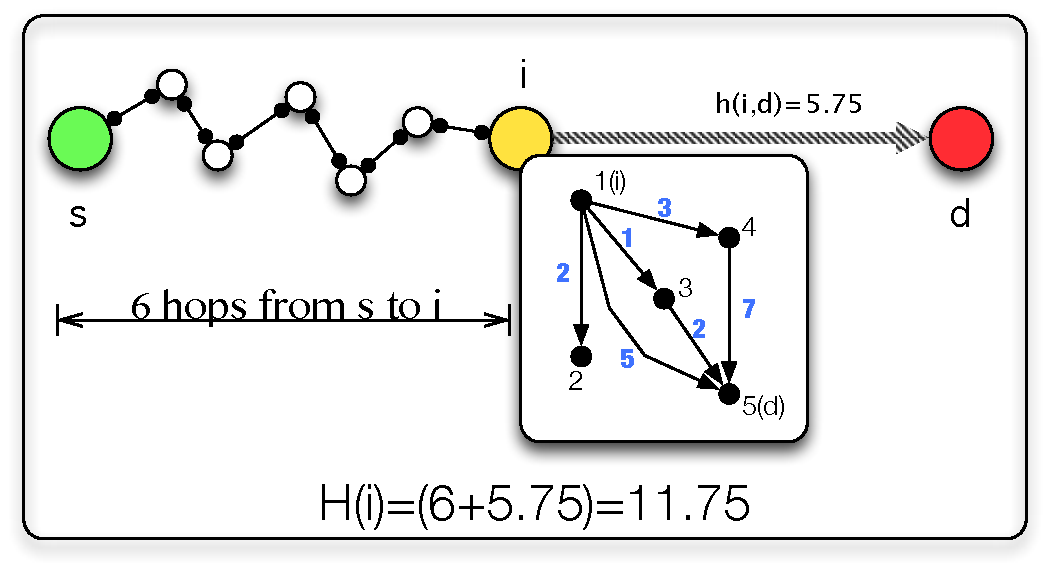
\includegraphics[width=0.6\textwidth]{paper-HCH/heuristic}
  \caption{跳数计算过程}
  \label{fig:chap5_heuristic}
\end{figure}

\figurename~\ref{fig:chap5_heuristic}展示了消息从源节点到目的节点跳数的估计过程。假设消息$M_k$在源节点$s$产生,目的节点为$d$,$i$是当前运行算法的节点。对于消息$M_k$而言,从节点$s$到$i$一共经过了6跳,因此有$hop(k)=6$。为了简便起见,在图中,当前节点$i$标号为$1$,目的节点$d$标号为5,如\figurename~\ref{fig:chap5_heuristic}所示。对于内层循环的首次迭代,有
\begin{displaymath}
M=\Lambda\bigodot A=\left(
\begin{array}{ccccc}
 0 & 2 & 1 & 3 & 5 \\ 
 0 & 0 & 0 & 0 & 0 \\
 0 & 0 & 0 & 0 & 2 \\
 0 & 0 & 0 & 0 & 7 \\
 0 & 0 & 0 & 0 & 0 \\
\end{array}
\right)
\end{displaymath}
其中,有
\begin{gather*}
m_{i,d}=m_{1,5}=5 \\
h = 0+5 = 5 \\
c = 0+1 = 1  
\end{gather*}
对于第二次迭代,有
\begin{displaymath}
M=A\bigodot A = \left(
\begin{array}{ccccc}
 0 & 0 & 0 & 0 & 6.5 \\ 
 0 & 0 & 0 & 0 & 0 \\
 0 & 0 & 0 & 0 & 0 \\
 0 & 0 & 0 & 0 & 0 \\
 0 & 0 & 0 & 0 & 0 \\
\end{array}\right)
\end{displaymath}
其中,有
\begin{gather*}
m_{i,d}=m_{1,5}=\left.[0+0+(1+2)+(3+7)+0]\right/2=6.5 \\
h=5+6.5=11.5 \\
c=1+1=2 
\end{gather*}
循环将在第三次迭代开始之前结束,因为元素$m_{i,d}=m_{1,5}=0$,最终得到如下结果
\begin{displaymath}
h(i,d)=\frac{h}{c}=\frac{11.5}{2}\approx 5.75
\end{displaymath}
注意上述计算结果$h(i,d)$是公式(\ref{eq:h})的一个近似值。在\figurename~\ref{fig:chap5_heuristic}所示例子中,通过公式(\ref{eq:h})可得平均跳数值为6,接近于计算结果5.75。


\section{路由协议}
\label{chap5:路由协议}

\begin{table}[bt]
  \caption{机会路由决策}
  \label{tab:chap5_routing}
  \centering
  \begin{tabular}{cc}
  \hline
   \textbf{策略:持有该消息的节点} & \textbf{对应情况}  \\
    \hline
    节点v和节点u & 向网络中增加一个新的消息副本\\
    节点v & 节点u不如节点v优\\
    节点u & 节点u比节点v优\\
    \hline
  \end{tabular}
\end{table}

\tablename~\ref{tab:chap5_routing}展示了两个相遇的节点可选的转发策略。在本章路由中,第一条原则是不刻意减少在网络中产生的副本数量。第二条原则旨在将网络中副本数量控制在一定范围之内,即当且仅当相遇的两个节点$u$和$v$都难以将数据包转发到目的节点时,才向网络中注入新的副本。在这种情况下,多拷贝策略被用来提高路由性能表现;在其它情况,只会在$u$和$v$之间选取唯一节点作为中继节点。

\begin{algorithm}[tbp] %算法的开始
\renewcommand{\algorithmicrequire}{\textbf{For}}
\caption{Routing} %算法的标题
\label{alg:chap5_routing} %给算法一个标签,这样方便在文中对算法的引用
\begin{algorithmic}[1] %这个1 表示每一行都显示数字
\REQUIRE each node $v\in V$ \textbf{do}
\STATE $neighbors\leftarrow v.getNeighbors()$
\FOR{$M_k\in v.messages$}
    \FOR{$u\in neighbors$}
        \STATE $s\leftarrow M_k.getSourceID()$
        \STATE $d\leftarrow M_k.getDestinationID()$
        \IF{$\mathcal{H}(v,k),\mathcal{H}(u,k)>\overline{hop}(s,d)$}
            \STATE $extra\leftarrow$ \textbf{true}
        \ELSE
            \STATE $extra\leftarrow$ \textbf{false}
        \ENDIF
        \IF{$extra=$ \textbf{true}}
            \STATE $v$ sends an extra copy of $M_k$ to $u$          
        \ELSIF{$\mathcal{H}(u,k)\leq \overline{hop}(s,d)$}
            \STATE $v$ turns over its own copy of $M_k$ to $u$
        \ENDIF
    \ENDFOR
\ENDFOR
\end{algorithmic}
\end{algorithm}

算法~\ref{alg:chap5_routing}为路由细节过程。如第1行所示,首先从当前节点$v$取得其邻居节点集合。然后,如2--16行所示,对存于节点$v$缓存中的每条消息,及所有其邻居节点做出路由决策。决策基于\label{chap5:启发函数}小节中的启发函数做出。考虑消息$M_k$,设其源节点为$s$目的节点为$d$。在$\mathcal{H}(v,k)$, $\mathcal{H}(u,k)$的值皆大于$\overline{hop}(s,d)$时,当前节点$v$及其邻居节点$u$其估计跳数皆大于$s$与$d$之间的平均跳数,这意味着对于节点$v$和$u$将消息在平均跳数之内传输至目的节点都很困难,此时多拷贝策略将被触发。

在6--10行,根据$extra$指示变量选择是否加入新的消息$M_k$的拷贝。若$extra=true$,$v$对节点$u$产生一份额外的$M_k$的拷贝,如第12行所示,这对应\tablename~\ref{tab:chap5_routing}的第一行策略。在第13--15行,若$\mathcal{H}(u,k)\leq\overline{hop}(s,d)$,节点$v$将把$M_k$移交给节点$u$,并将其从$v$中缓存移除。在这种情况下,有$\mathcal{H}(u,k)\leq\mathcal{H}(v,k)\leq\overline{hop}(s,d)$;由此认为节点$u$足以将消息$M_k$递交于目的节点;对应\tablename~\ref{tab:chap5_routing}中第三条表目。剩下的唯一一种情况即$\mathcal{H}(v,k)\leq\mathcal{H}(u,k)\leq\overline{hop}(s,d)$,意味着节点$u$不是优于$v$的中继节点选择(针对消息$M_k$而言),且节点$v$自身足以将消息在平均时延内传递至目的节点。在该情况下,$v$不向$u$转发$M_k$,对应\tablename~\ref{tab:chap5_routing}条目二。

\section{仿真实验}
\label{chap5:仿真实验}

仿真实验基于机会网络模拟器ONE~\upcite{Keranen2009}。本章将提出的算法与Epidemic, Spray-and-Wait (S \& W)以及PRoPHET相比较,仿真实验场景包含Helsinki City Model以及Cambridge-iMote。实验可分为如下几组:Helsinki City Model下改变节点缓存大小;Cambridge-iMote下改变节点缓存大小;Helsinki City Model下改变消息TTL;Cambridge-iMote下改变消息TTL。仿真评估标准分为消息投递率,平均时延,网络开销三项。

\subsection{Helsinki City场景}



\begin{table}
\centering
\caption{Helsinki City场景仿真设置}
\label{tab:chap5_simulation_helsinki}
\begin{tabular}{
p{0.45\linewidth}<{\centering}
p{0.5\linewidth}<{\centering}
}
\hline
\textbf{parameter name} & \textbf{range(default value)} \\
\hline
number of nodes & 120  \\
world size($m\times m$) & 4500$\times$3000  \\
tickets for S \& W & 13 \\
message TTL(min) & 200--500 (300) \\
simulation time(hours) & 12 \\
message size(KB) & 500--1024 \\
pedestrian buffer(MB) & 15--55 (15) \\
tram buffer(MB) & 500 \\
bluetooth range(m) & 10 \\
highspeed range(m) & 1000 \\ 
bluetooth bandwidth(KBps) & 250 \\
highspeed bandwidth(MBps) & 10 \\ 
pedestrian speed(m/s) & 0.5--1.5  \\
message interval(s) & 35--40 \\
\hline
\end{tabular}
\end{table}

仿真参数设置如\tablename~\ref{tab:chap5_simulation_helsinki}所示。对于\figurename~\ref{fig:chap5_helsinki_buffer}(a),\ref{fig:chap5_helsinki_buffer}(b)与\ref{fig:chap5_helsinki_buffer}(c)所示实验结果,本章提出的HCH算法具有最高的投递率以及最低的投递时延。HCH算法的网络开销比S \& W高,但比Epidemic及PRoPHET依然低很多。\figurename~\ref{fig:chap5_helsinki_buffer}(a)所示结果,HCH算法在投递率方面的表现优于PRoPHET以及Epidemic很多,略优于S \& W。如\figurename~\ref{fig:chap5_helsinki_buffer}(b)所示,HCH的平均投递时延比Epidemic及PRoPHET低,比S \& W略低。由于HCH利用启发式方法估计平均跳数,从而自适应地利用多拷贝策略进行路由,避免了一些不必要的网络消息副本冗余。HCH算法所产生的副本数量,要比Epidemic以及PRoPHET少很多。为了投递某条消息,所需要的消息副本数量越少,则意味着越高的投递效率。HCH算法具有比Epidemic以及PRoPHET低很多的网络开销,如\figurename\ref{tab:chap5_simulation_helsinki}(c)所示。从\figurename\ref{tab:chap5_simulation_helsinki}(c)可以看出,S\& W的网络开销小于HCH, 然而在投递率和平均时延方面,HCH皆优于S \& W。

\begin{figure*}[tbp]
\centering
\subfigure[buffer size vs delivery\label{helsinki_delivery_buffer}]
{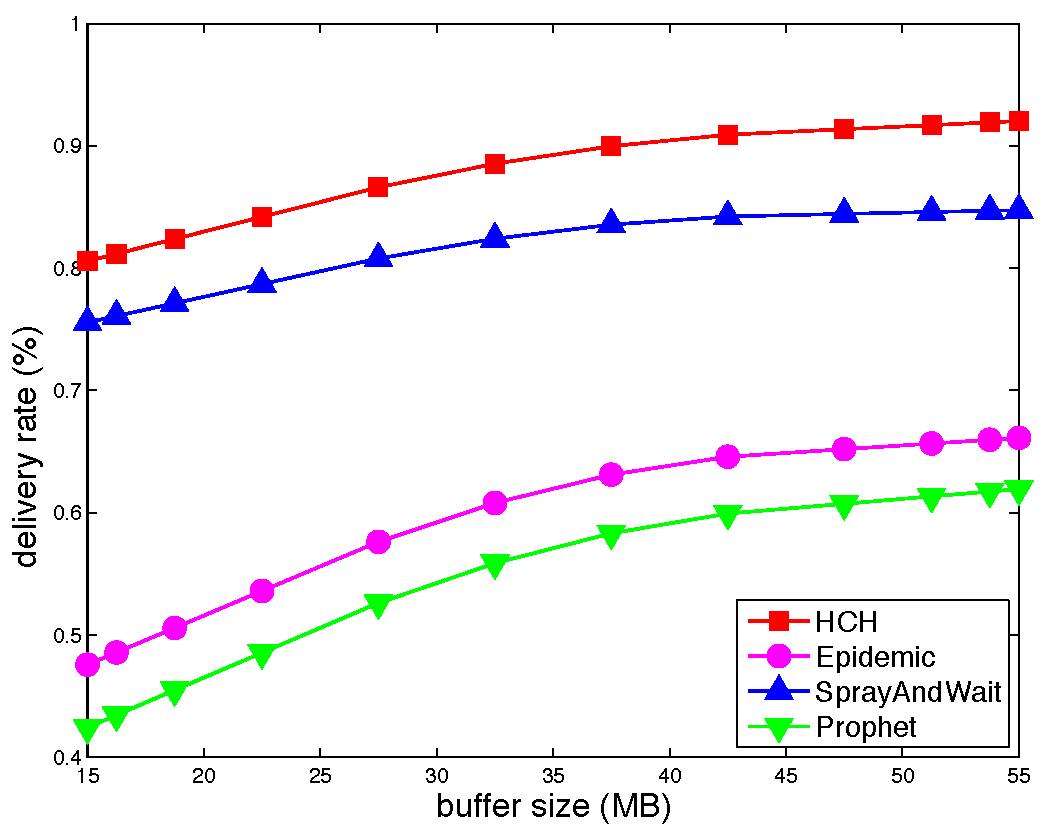
\includegraphics[width=0.32\linewidth]{paper-HCH/helsinki_delivery_buffer}}
\subfigure[buffer size vs latency\label{helsinki_latency_buffer}]
{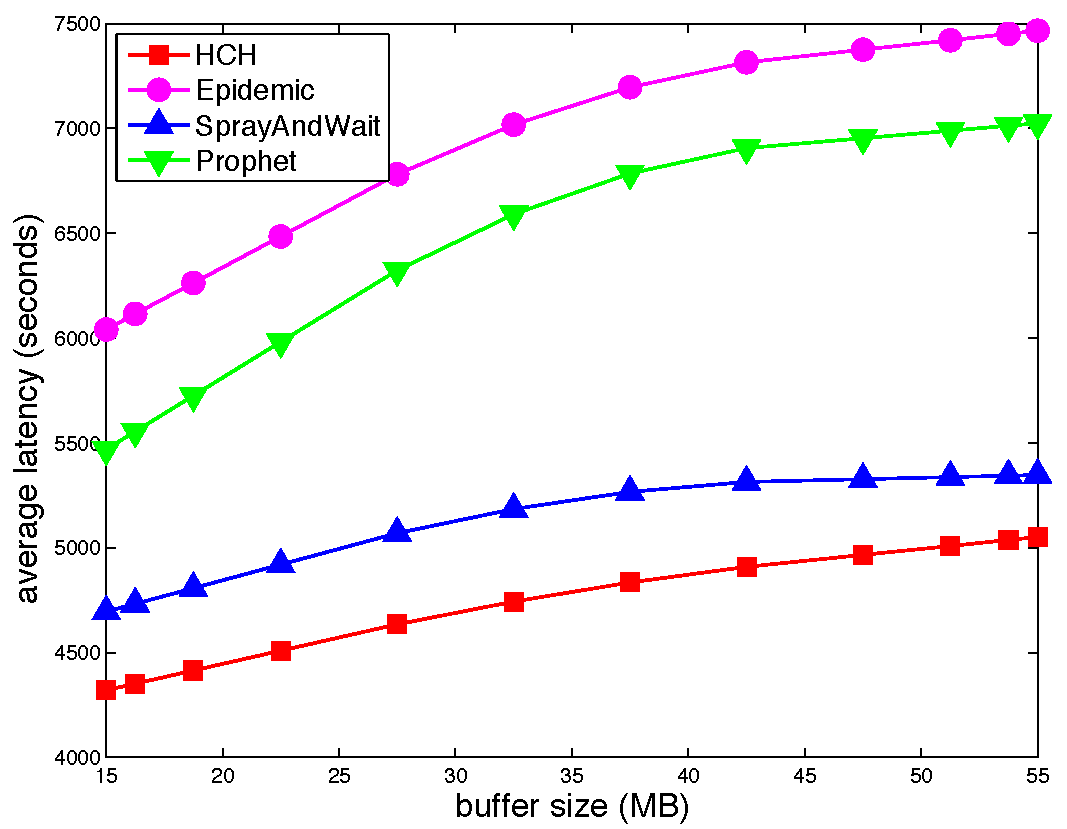
\includegraphics[width=0.32\linewidth]{paper-HCH/helsinki_latency_buffer}}
\subfigure[buffer size vs overhead\label{helsinki_overhead_buffer}]
{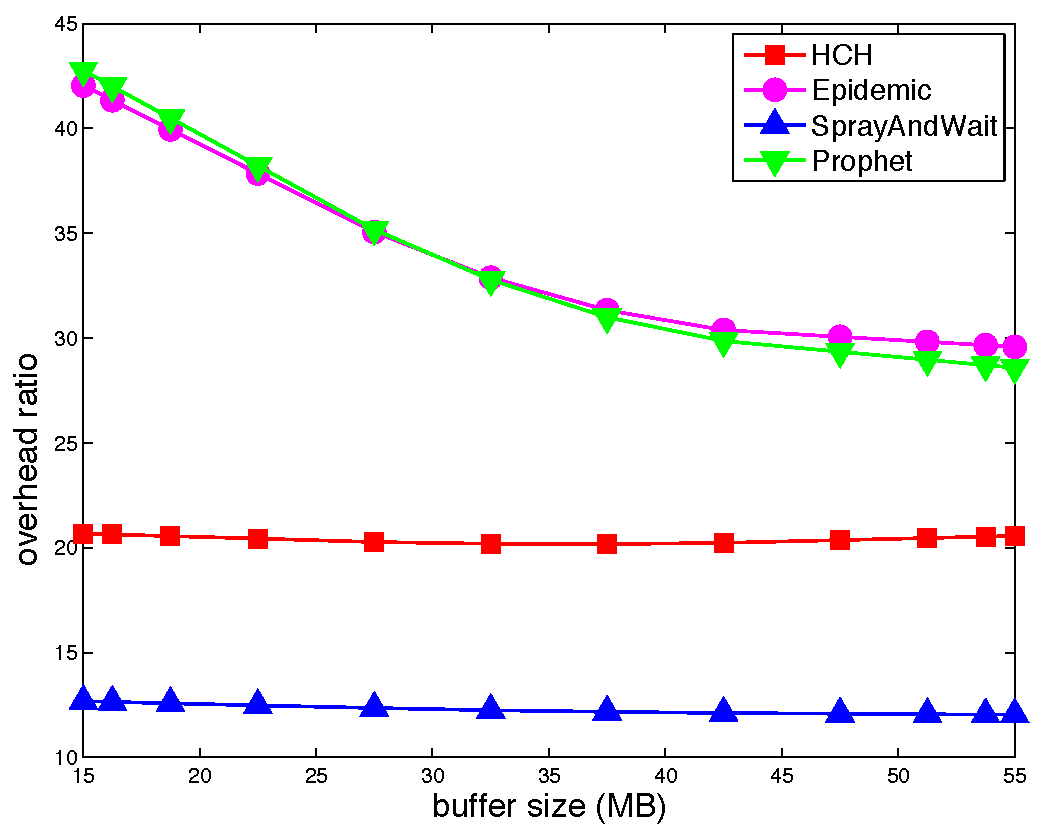
\includegraphics[width=0.32\linewidth]{paper-HCH/helsinki_overhead_buffer}}
\caption{[\emph{Helsinki City Scenario}] 改变节点缓存大小的仿真结果}
\label{fig:chap5_helsinki_buffer}
\end{figure*}


在改变消息TTL的仿真中,节点的缓存大小(只针对行人和轿车,对电车不做设置)设为15 MB。\figurename~\ref{fig:chap5_helsinki_ttl}(a)所示仿真结果中,HCH在投递率方面的表现优于其它三种算法。HCH的平均时延在所有算法中保持最低,如\figurename~\ref{fig:chap5_helsinki_ttl}(b)所示。此外如\figurename~\ref{fig:chap5_helsinki_ttl}(c),HCH在网络开销方面具有较好的表现。\figurename~\ref{fig:chap5_helsinki_ttl}(a)的结果表明,当节点缓存资源受限时,洪泛路由策略不适用。其余两种基于洪泛的路由算法,其投递率亦较低,这是由于受限的缓存资源导致了较高的丢包率。HCH性能表现在四种路由算法中最优。此外,当消息的TTL设为大于250分钟时,HCH的平均时延比S \& W低,结果如\figurename~\ref{fig:chap5_helsinki_ttl}(b)所示。从\figurename~\ref{fig:chap5_helsinki_ttl}(a),\ref{fig:chap5_helsinki_ttl}(b)以及\ref{fig:chap5_helsinki_ttl}(c)可以看出,在此仿真中,消息的TTL对路由性能表现影响较小。


\begin{figure*}[tbp]
\centering
\subfigure[message TTL vs delivery\label{helsinki_delivery_ttl}]
{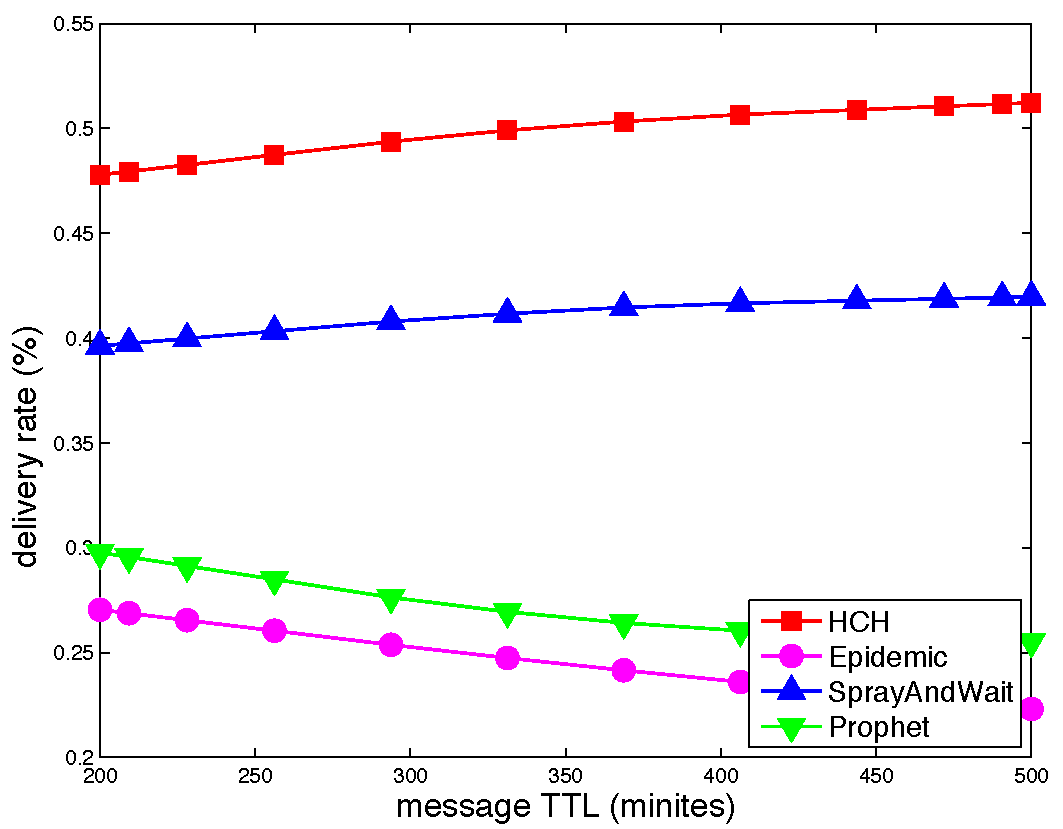
\includegraphics[width=0.32\linewidth]{paper-HCH/helsinki_delivery_ttl}}
\subfigure[message TTL vs latency\label{helsinki_latency_ttl}]
{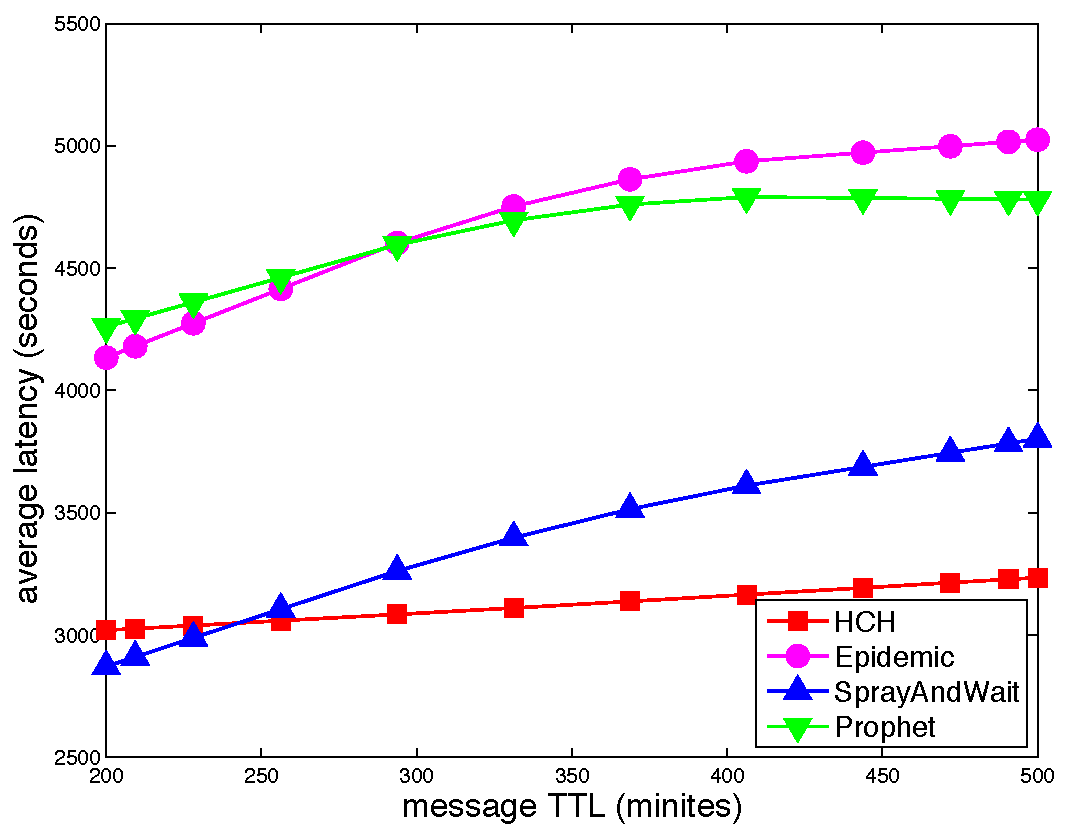
\includegraphics[width=0.32\linewidth]{paper-HCH/helsinki_latency_ttl}}
\subfigure[message TTL vs overhead\label{helsinki_overhead_ttl}]
{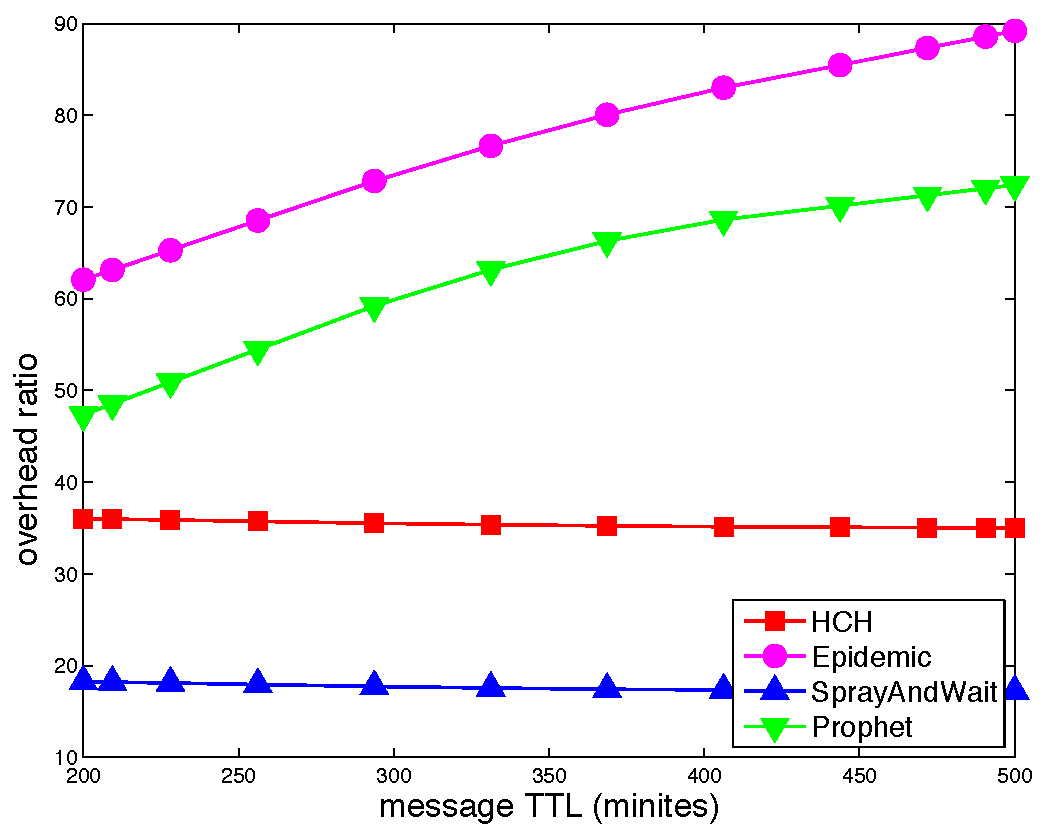
\includegraphics[width=0.32\linewidth]{paper-HCH/helsinki_overhead_ttl}}
\caption{[\emph{Helsinki City Scenario}] 改变消息TTL的仿真结果}
\label{fig:chap5_helsinki_ttl}
\end{figure*}



\subsection{Cambridge-iMote场景}

\begin{table}[tbp]
\centering
\caption{Simulation settings of Cambridge-iMote trace}
\label{tab:chap5_simulation_trace}
\begin{tabular}{
p{0.45\linewidth}<{\centering}
p{0.5\linewidth}<{\centering}
}
\hline
\textbf{parameter name} & \textbf{range} \\
\hline
number of nodes & 36  \\
tickets for S \& W & 5  \\
message TTL(min) & 600--2000(1200) \\
simulation time(days) & 11.5 \\
message size(KB) & 500--1024 \\
device buffer(MB) & 50--150(100) \\
interface bandwidth(KBps) & 250 \\
message interval(s) & 35--40 \\
\hline
\end{tabular}
\end{table}

仿真实验如\tablename~\ref{tab:chap5_simulation_trace}所示。在真实数据集的仿真中,缓存大小的设置值相比Helsinki City Scenario要大许多。\figurename~\ref{fig:chap5_trace_buffer}(a)显示HCH的投递率约与Epidemic相同。当缓存大小设为大于110 MB时,HCH在投递率方面由于PRoPHET。如\figurename~\ref{fig:chap5_trace_buffer}(b)所示结果,HCH的投递时延比S \& W高,比PRoPHET以及Epidemic低很多。S \& W算法投递时延低的原因是其计入统计的消息副本数量极其少,因为其成功投递的消息副本数量很少,如\figurename~\ref{fig:chap5_trace_buffer}(a)结果所示。在其路由过程中,有大量在到达目的节点前即被丢弃的消息数据包存在。集中比较Epidemic, PRoPHET,HCH三种算法可以发现,即使HCH的投递率表现相比PRoPHET优势不明显,劣于Epidemic时,其投递时延的性能表现优于该两种基于洪泛的路由算法。此外,从\figurename~\ref{fig:chap5_trace_buffer}(c)可以看出,Epidemic具有最高的网络开销,意味着更多的网络资源将会被消耗。


\begin{figure*}[tbp]
\centering
\subfigure[buffer size vs delivery\label{realtrace_delivery_buffer}]
{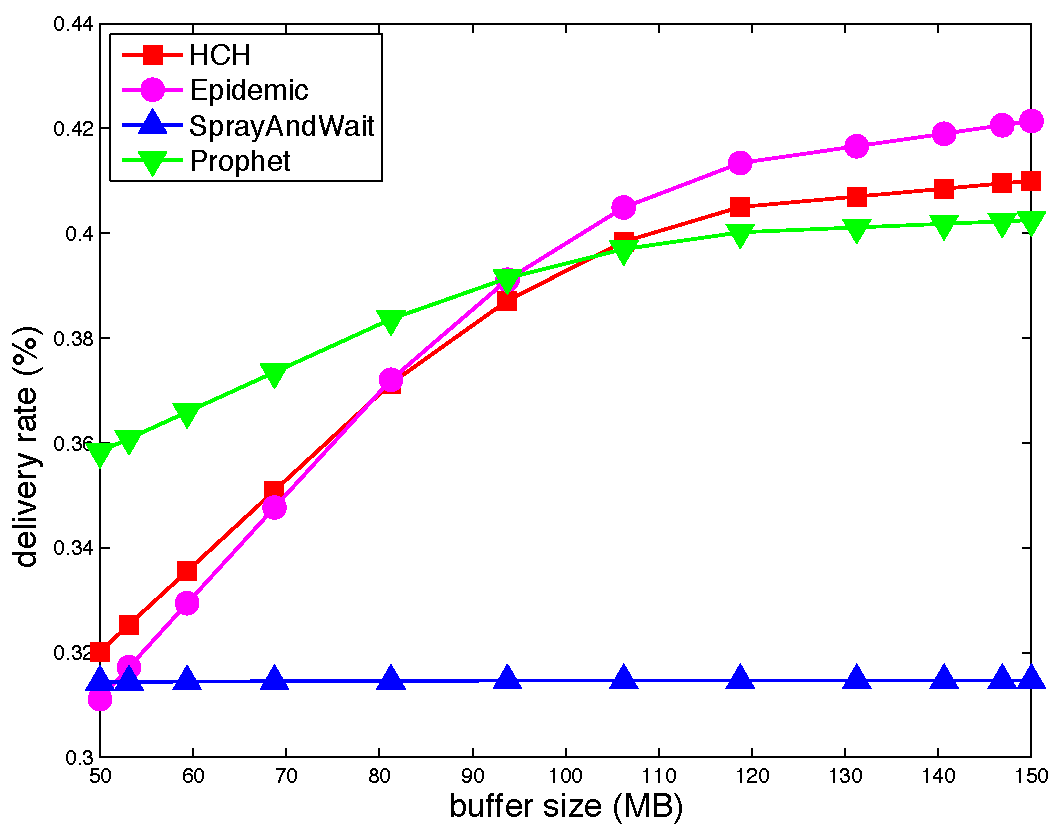
\includegraphics[width=0.32\linewidth]{paper-HCH/realtrace_delivery_buffer}}
\subfigure[buffer size vs latency\label{realtrace_latency_buffer}]
{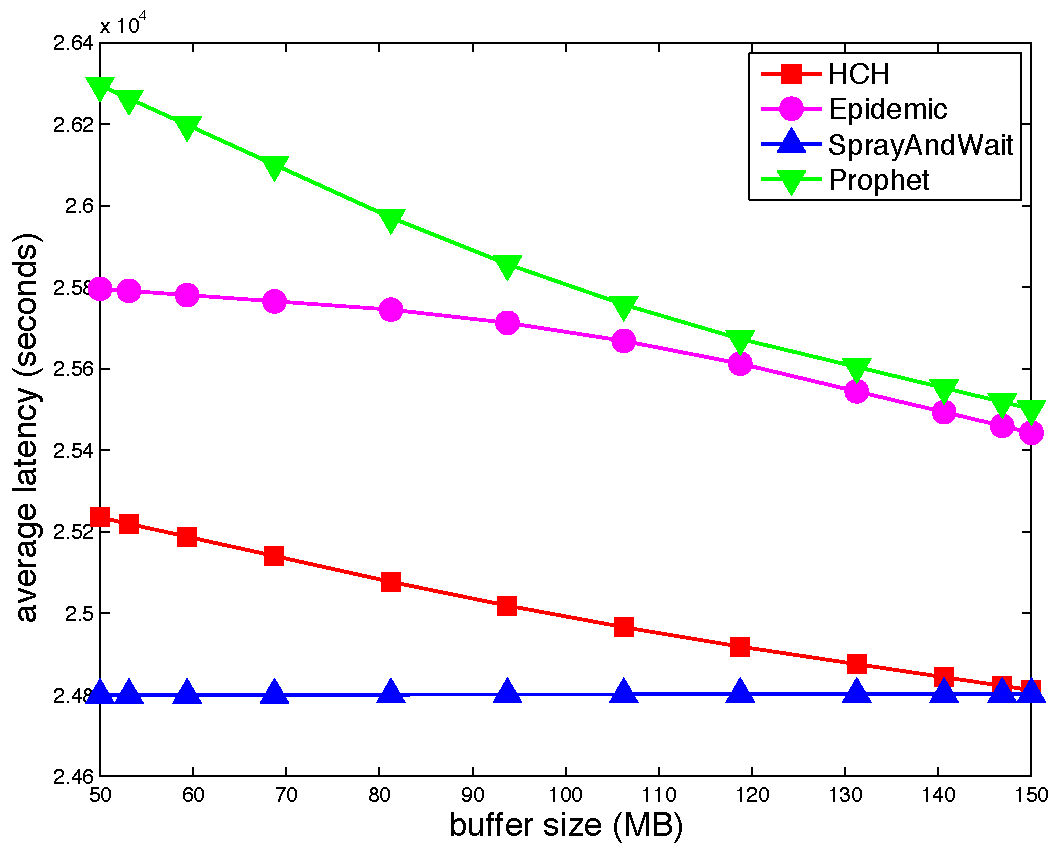
\includegraphics[width=0.32\linewidth]{paper-HCH/realtrace_latency_buffer}}
\subfigure[buffer size vs overhead\label{realtrace_overhead_buffer}]
{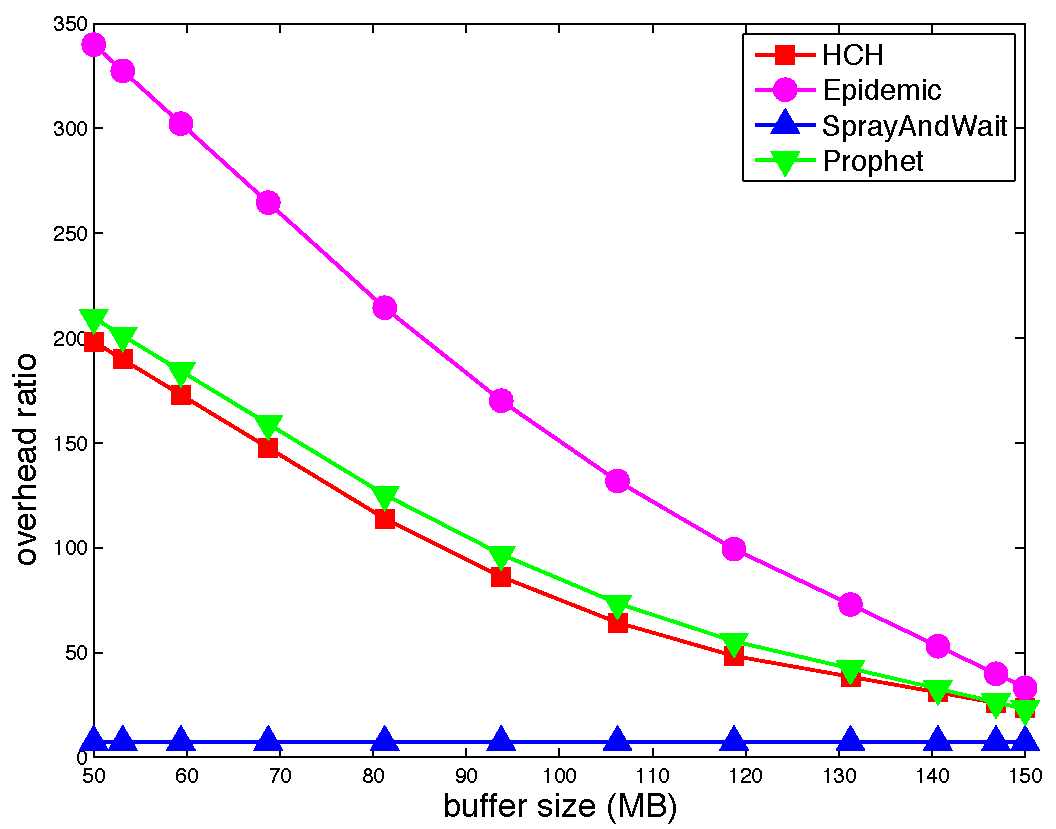
\includegraphics[width=0.32\linewidth]{paper-HCH/realtrace_overhead_buffer}}
\caption{[\emph{Cambridge-iMote}] Buffer size vs delivery ratio, average latency and overhead ratio.}
\label{fig:chap5_trace_buffer}
\end{figure*}

在\figurename~\ref{fig:chap5_realtrace_ttl}所示的仿真中,节点的缓存大小设为100 MB。如\figurename~\ref{fig:chap5_realtrace_ttl}(a)所示,随着消息TTL值的增加,几种路由算法的投递率性能表现都上升。然而在Epidemic, PRoPHET以及HCH三者中,投递率表现并无明显差异。从\figurename~\ref{fig:chap5_realtrace_ttl}(c)可见,HCH的网络开销仅比S \& W高一点,相比Epidemic以及PRoPHET却低很多。\figurename~\ref{fig:chap5_realtrace_ttl}(b)中结果显示,所有四种算法在投递时延方面拥有几乎一样的性能表现。当消息TTL设为较大值时,所有算法都具有相对较高的投递时延,投递率也随之上升。比较\figurename~\ref{fig:chap5_realtrace_ttl}(a)及\ref{fig:chap5_realtrace_ttl}(b)所示结果,随着消息TTL值增大,投递时延上升速度比投递率快很多。由此可推断出在此种情况下,网络中某些消息在短期之内很难完成投递。


\begin{figure*}[tbp]
\centering
\subfigure[message TTL vs delivery\label{realtrace_delivery_ttl}]
{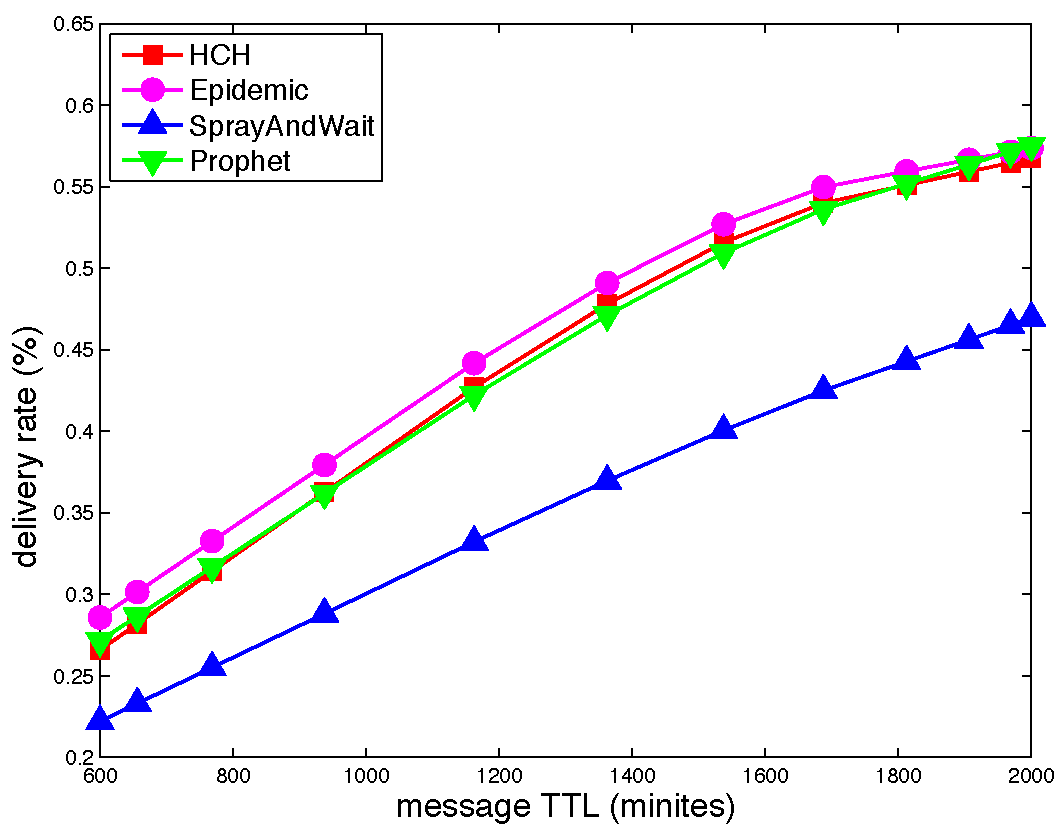
\includegraphics[width=0.32\linewidth]{paper-HCH/realtrace_delivery_ttl}}
\subfigure[message TTL vs latency
\label{realtrace_latency_ttl}]
{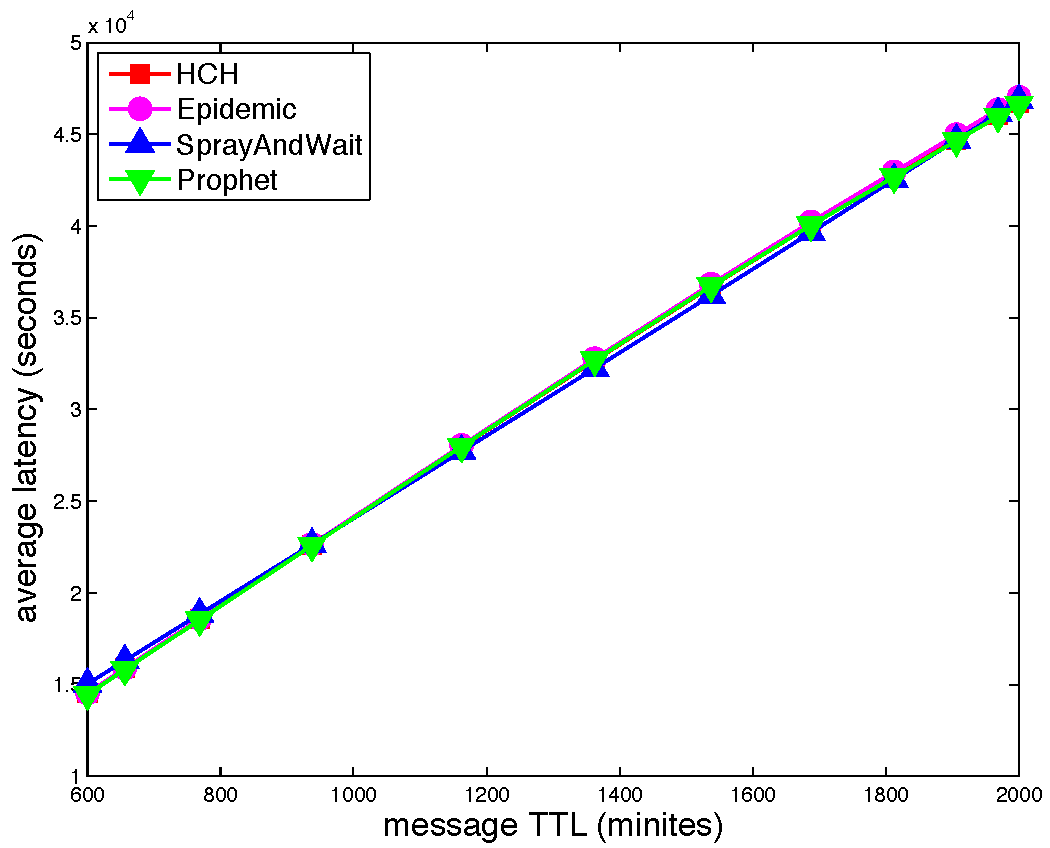
\includegraphics[width=0.32\linewidth]{paper-HCH/realtrace_latency_ttl}}
\subfigure[message TTL vs overhead\label{realtrace_overhead_ttl}]
{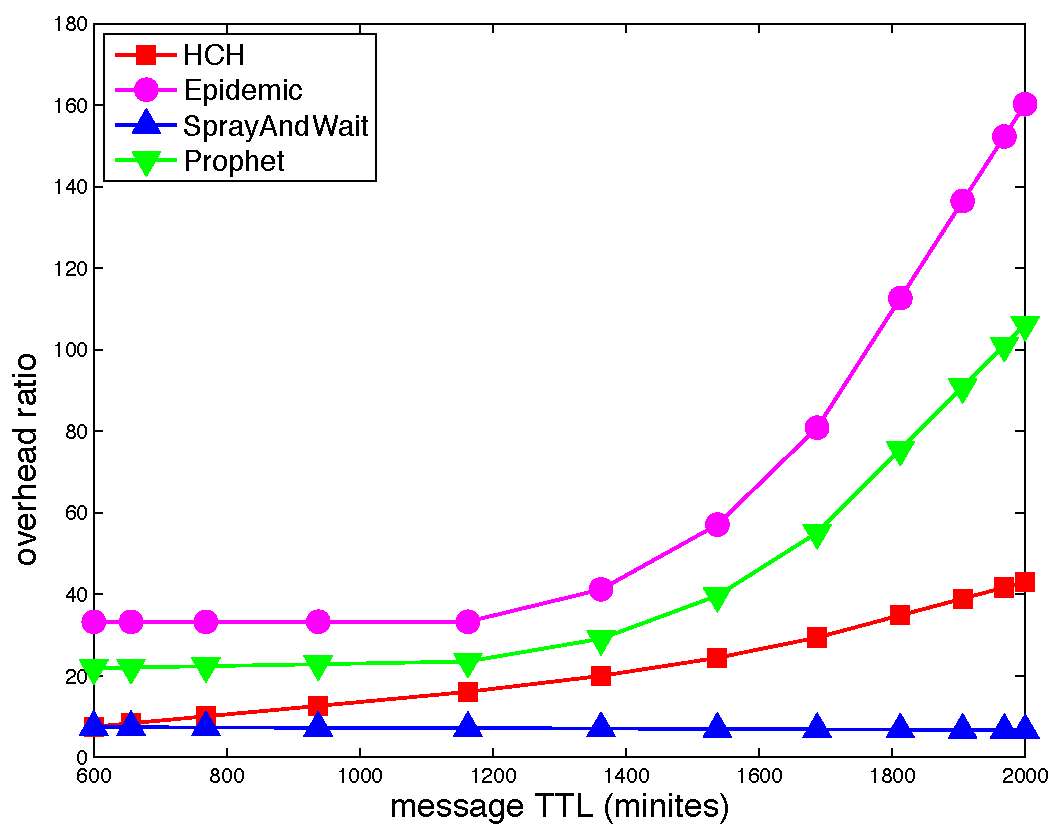
\includegraphics[width=0.32\linewidth]{paper-HCH/realtrace_overhead_ttl}}
\caption{[\emph{Cambridge-iMote}] Message TTL vs delivery ratio, average latency and overhead ratio.}
\label{fig:chap5_realtrace_ttl}
\end{figure*}

总之,从Helsinki City Scenario仿真可以看出,HCH算法在投递时延以及网络开销方面具有明显优势。此外,HCH是在两类仿真场景中唯一一个都具有良好投递率的算法。

\section{本章小结}
\label{chap5:本章小结}

本章提出了一种基于跳数的启发式路由协议HCH,利用启发函数,基于跳数信息进行消息投递跳数预测。利用滑动窗口机制,可以动态更新记录平均跳数的矩阵。基于此,定义了启发式函数用于预测当前节点到目的节点之间的潜在跳数。为了便于计算,定义了一种矩阵运算符,从而将跳数的估计过程转化为矩阵运算。仿真实验表明,本章提出的HCH算法在综合性能表现上优于Epidemic, S \& W以及PRoPHET。
